\documentclass{article}
\usepackage[MeX]{polski}
\usepackage[utf8]{inputenc}
\usepackage{listings}
\usepackage{xcolor}
\usepackage{graphicx}
\usepackage[margin=1in,footskip=0.25in]{geometry}
\usepackage{float}
\usepackage{subfigure}

\renewcommand\thesubsubsection{\textbf{\alph{subsubsection}})}


\pagestyle{plain}

\author{Tymon Kwiatkowski - 319272\\
    Konrad Kotlicki - 310958\\
    Adam Fedorowicz - 319266\\}


\date{Styczeń 2022}
\title{Sprawozdanie z empirycznej analizy algorymów sortowania}

\begin{document}

\definecolor{codegreen}{rgb}{0,0.6,0}
\definecolor{codegray}{rgb}{0.5,0.5,0.5}
\definecolor{codepurple}{rgb}{0.58,0,0.82}
\definecolor{backcolour}{rgb}{0.95,0.95,0.92}
\lstdefinestyle{mystyle}{
    backgroundcolor=\color{backcolour},
    commentstyle=\color{codegreen},
    keywordstyle=\color{magenta},
    numberstyle=\tiny\color{codegray},
    stringstyle=\color{codepurple},
    basicstyle=\ttfamily\footnotesize,
    breakatwhitespace=false,
    breaklines=true,
    captionpos=b,
    keepspaces=true,
    numbers=left,
    numbersep=5pt,
    showspaces=false
    showstringspaces=false,
    showtabs=false,
    tabsize=2
}
\lstset{style=mystyle}

\maketitle

\begin{flushleft}
Przedmiot: Algorytmy i Struktury Danych\\
Kierunek: Geoinformatyka\\
Rok Akademicki: 2021Z semestr I\\
Tytuł Ćwiczenia: Sortowanie Shella a sortowanie przez scalanie
\end{flushleft}

\tableofcontents
\thispagestyle{empty}
\break

\clearpage
\pagenumbering{arabic} 
\section{Wstęp}

\subsection{Przedstawienie celu zadania}
\paragraph{} Celem badania jest zaimplementowanie oraz zaobserwowanie różnic między sortowaniem Shella, a sortowaniem przez scalanie.\\
Do tego celu przeprowadzone zostały testy działania tych algorytmów na tablicach:\\
•	losowych\\
•	posortowanych\\
•	posortowanych malejąco\\
•	prawie posortowanych\\
O liczbie  elementów wynoszącej od \textbf{50 tys} do \textbf{10 mln}. \\

\textbf{Wyniki tych testów mają nam również pomóc w odpowiedzeniu na poniższe pytania:}\\
•	Dla jakich wielkości tablicy sortowanie Shella działa z porównywalną prędkością, co sortowanie przez scalanie?\\
•	W jakich warunkach lepiej jest wykorzystać sortowanie Shella? Oraz do jakich zastosowań?

\break
\section{Analiza Algorytmów}

\subsection{Sortowanie Shella}

\subsubsection{Omówienie działania algorytmu}
\paragraph{} Sortowanie Shella bazuje na zasadzie podziału dużego problemu na mniejsze, łatwiejsze do rozwiązania. Duża tablica danych do posortowania jest dzielona na mniejsze rozłączne tablice zawierające, co ${h}$-ty element. W tak przygotowanych tablicach algorytm sortuje elementy sortowaniem przez wstawianie. Następnie algorytm wykonuje tą samą operacje, jednakże tym razem dla mniejszego h, aż do ${h = 1}$.

\subsubsection{Złożoność czasowa}
\paragraph{}Efektywność tego algorytmu zależna jest w dużym stopniu od przyjętego wzoru na ciąg wartości h. W pierwszych wersja tego algorytmu wzór ten wyglądał następująco ${h = \frac{1}{2}(k-1)}$ oraz dawał złożoność czasową ${\Theta(N^2 )}$.
W tym zadaniu wykorzystany został wzór ${h = \frac{1}{2}(3k-1)}$, którego złożoność czasowa jest wyrażona przez ${\Theta(N^\frac{3}{2})}$.

\subsubsection{Kod użyty w badaniu}
\begin{lstlisting}[language=C++]
// Exchanges values
inline void exch(int a[], int i, int j)
{
	int t = a[i];
	a[i] = a[j];
	a[j] = t;
}

// shell sort
void shell_sort(int a[], int size)
{
	int h = 1;
	while (h < size / 3)
	{
		h = 3 * h + 1; // 1, 4, 13, 40, 121, 364, ...
	}

	while (h >= 1)
	{
		for (int i = h; i < size; i++)
		{
			for (int j = i; j >= h; j -= h)
			{
				if (a[j] < a[j - h])
				{
					exch(a, j, j - h);
				}
				else
				{
					break;
				}
			}
		}

		h /= 3;
	}
}
\end{lstlisting}

\subsection{Sortowanie przez Scalanie}

\subsubsection{Omówienie działania algorytmu}
\paragraph{} Podobnie do Sortowania Shella sortowanie przez scalanie zasadzie "dziel i zwyciężaj", łatwiejsze do rozwiązania. Tablica wejściowych do posortowania jest dzielona na dwie części. Następnie dla każdej części wywoływane jest rekurencyjnie sortowanie przez scalanie. Gdy algorytm posortuje obie części, dwie takie tablice są scalane w jedną wyjściową, która jest już posortowana.

\subsubsection{Złożoność czasowa}
\paragraph{}Złożoność obliczeniowa algorytmu jest jednakowa dla przypadku najlepszego, średniego i najgorszego, i wynosi ${\Theta(Nlog(N))}$.


\subsubsection{Kod użyty w badaniu}
\begin{lstlisting}[language=C++]
// merge operation
void merge(int a[], int aux[], int lo, int mid, int hi)
{
	// copy
	for (int k = lo; k <= hi; k++)
	{
		aux[k] = a[k];
	}

	// merge
	int i = lo, j = mid + 1;
	for (int k = lo; k <= hi; k++)
	{
		if (i > mid)              a[k] = aux[j++]; // left array empty
		else if (j > hi)          a[k] = aux[i++]; // right array empty
		else if (aux[j] < aux[i]) a[k] = aux[j++]; // right value lower
		else                      a[k] = aux[i++]; // left value lower
	}
}

// merge sort
void merge_sort(int a[], int aux[], int lo, int hi)
{
	if (hi <= lo) return;       // stop when nothing to sort
	int mid = (lo + hi) / 2;    // find middle

	merge_sort(a, aux, lo, mid);      // sort left half  
	merge_sort(a, aux, mid + 1, hi);  // sort right half
	merge(a, aux, lo, mid, hi);       // merge arrays
}

// merge sort
void merge_sort(int a[], int size)
{
	int* aux = new int[size];
	merge_sort(a, aux, 0, size - 1);
	delete[] aux;
}
\end{lstlisting}
\break

\section{Sortowanie Shella a sortowanie przez scalanie}
\subsection{Przebieg ćwiczenia}
\paragraph{} Wygenerowaliśmy 800 plików z danymi o łącznym rozmiarze 29,1 GB. Po 200 tablic każdego z wymienionych we wstępie rodzajów. Tak wygenerowane zbiory posortowaliśmy obydwoma algorytmami oraz zmierzyliśmy czas każdego przypadku. Następnie na bazie tych danych stworzyliśmy wykresy, dzięki którym zaobserwowaliśmy zależności między sortowaniem Shella, a sortowaniem prze scalanie.

\subsection{Empiryczna analiza algorytmów}
\paragraph{} Poniżej umieściliśmy wykresy przedstawiające czas w sekundach jaki zajęło algorytmom posortowanie tablic liczb o rosnącej liczbie elementów.

\begin{figure}[H]
\caption{}
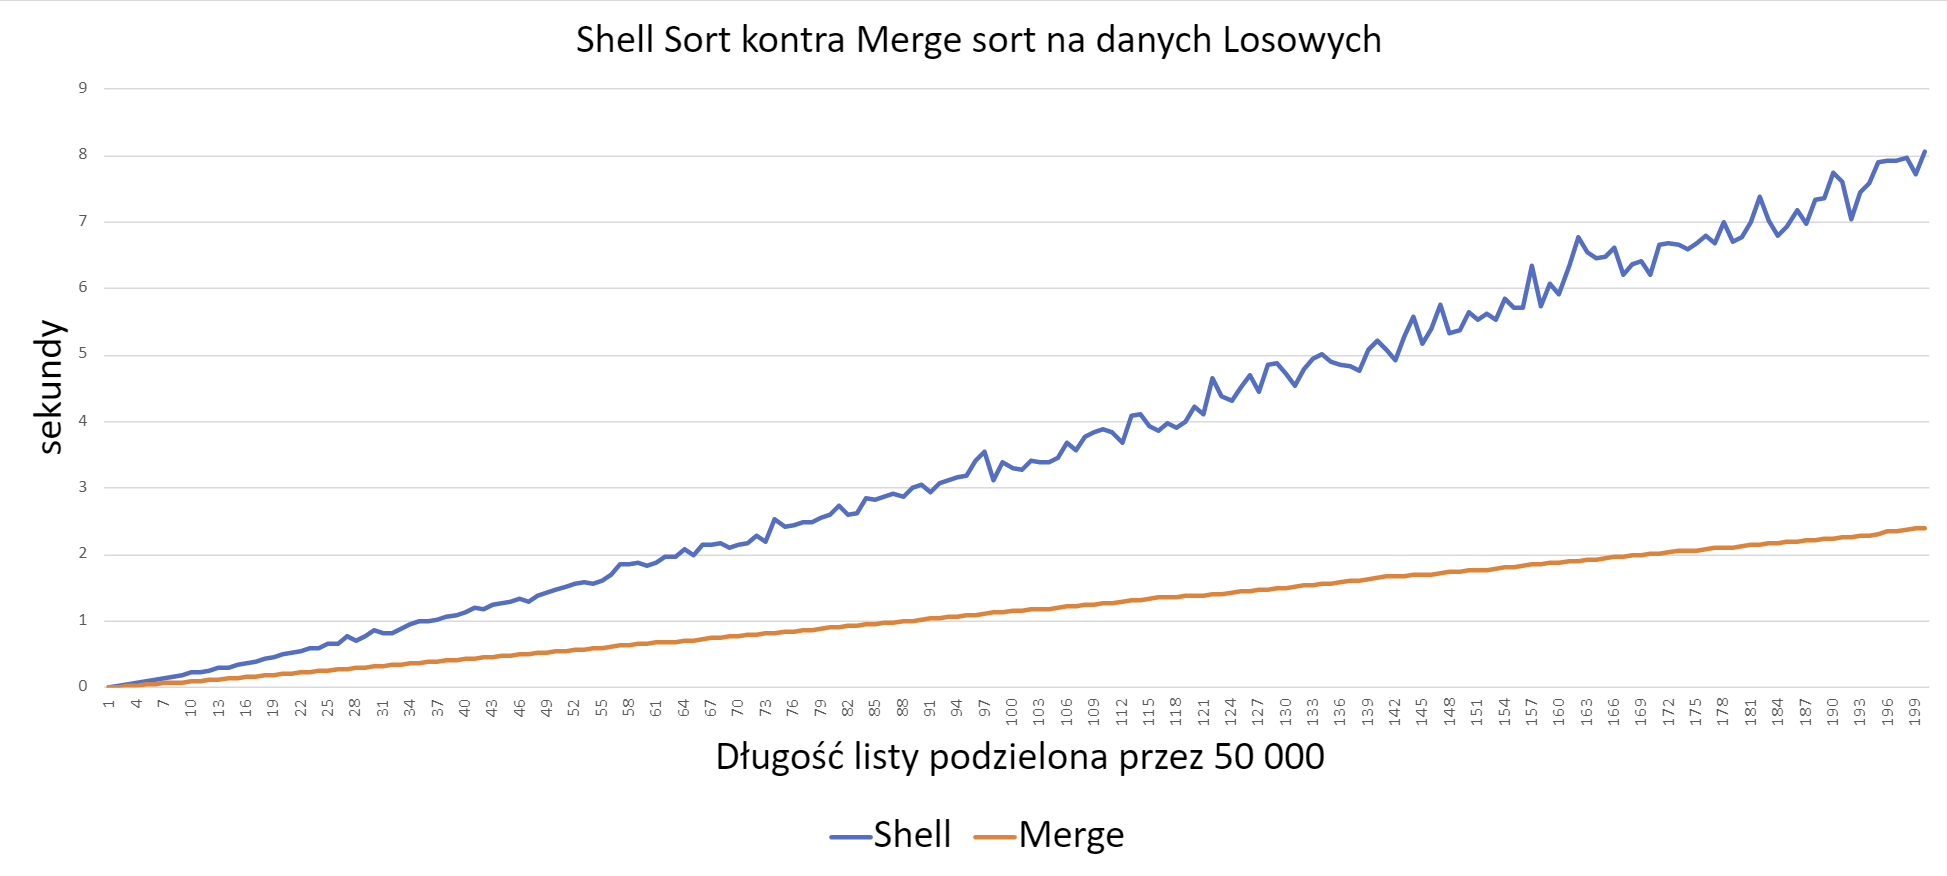
\includegraphics[scale = 0.23]{rand_f.png}\\
\caption{}
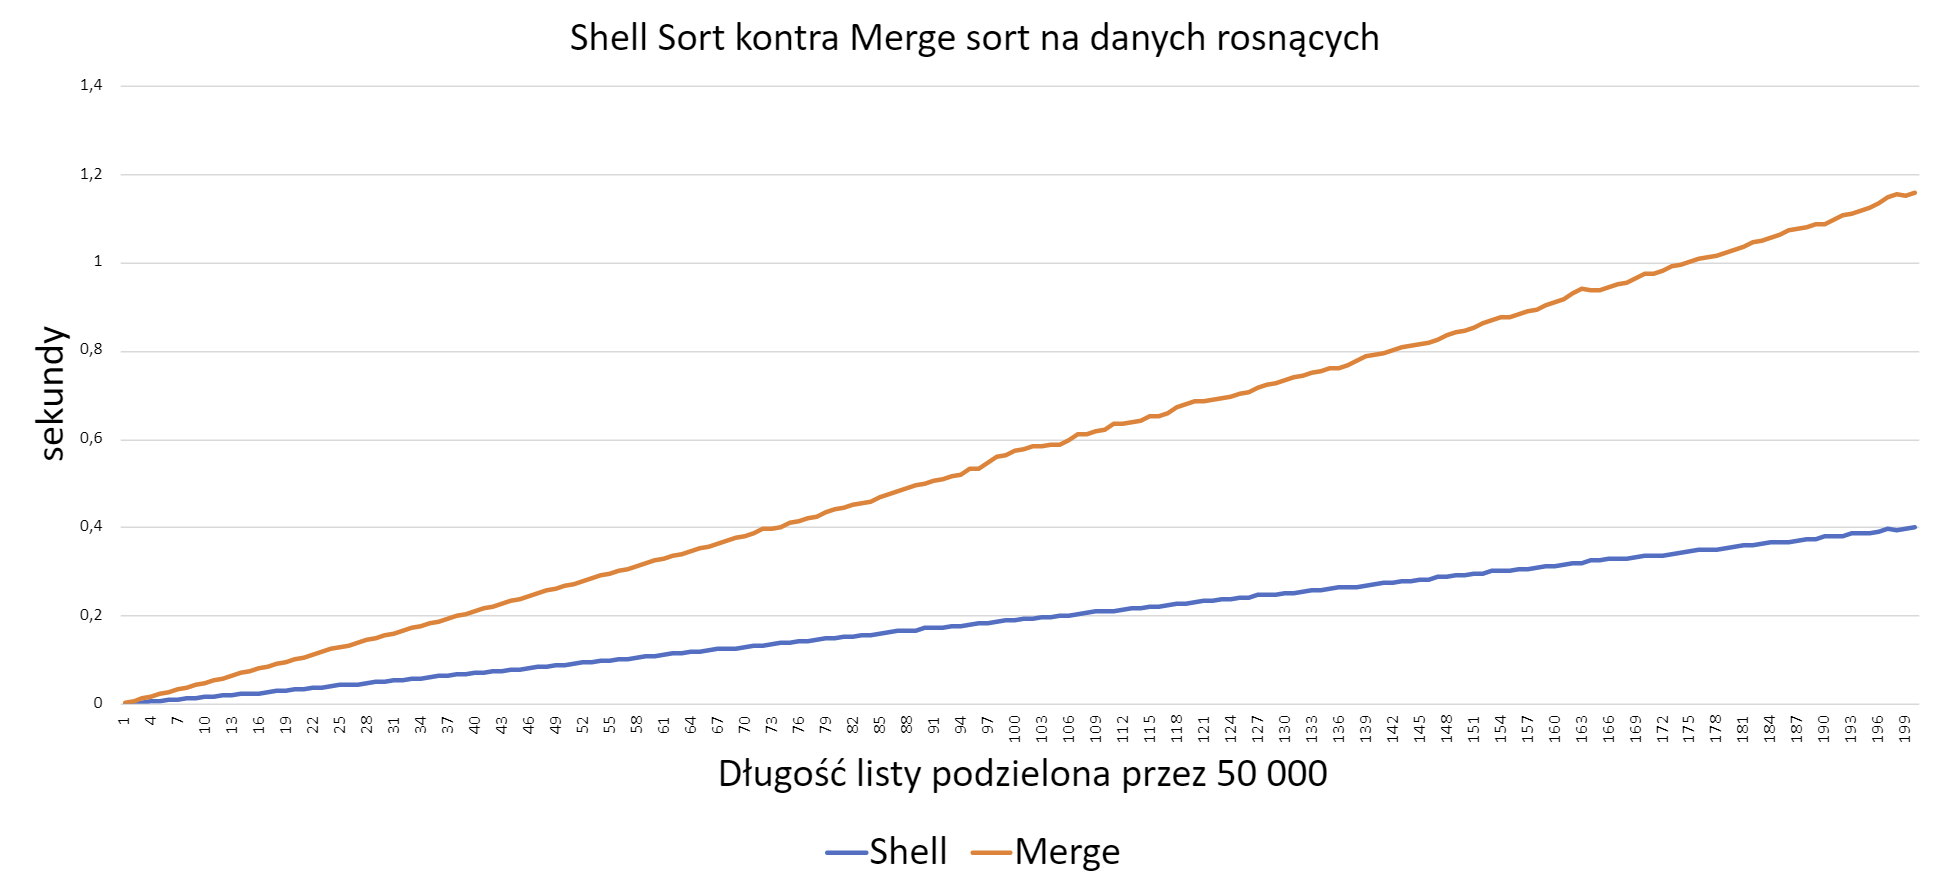
\includegraphics[scale = 0.23]{rise_f.png}\\
\end{figure}
\begin{figure}[H]
\caption{}
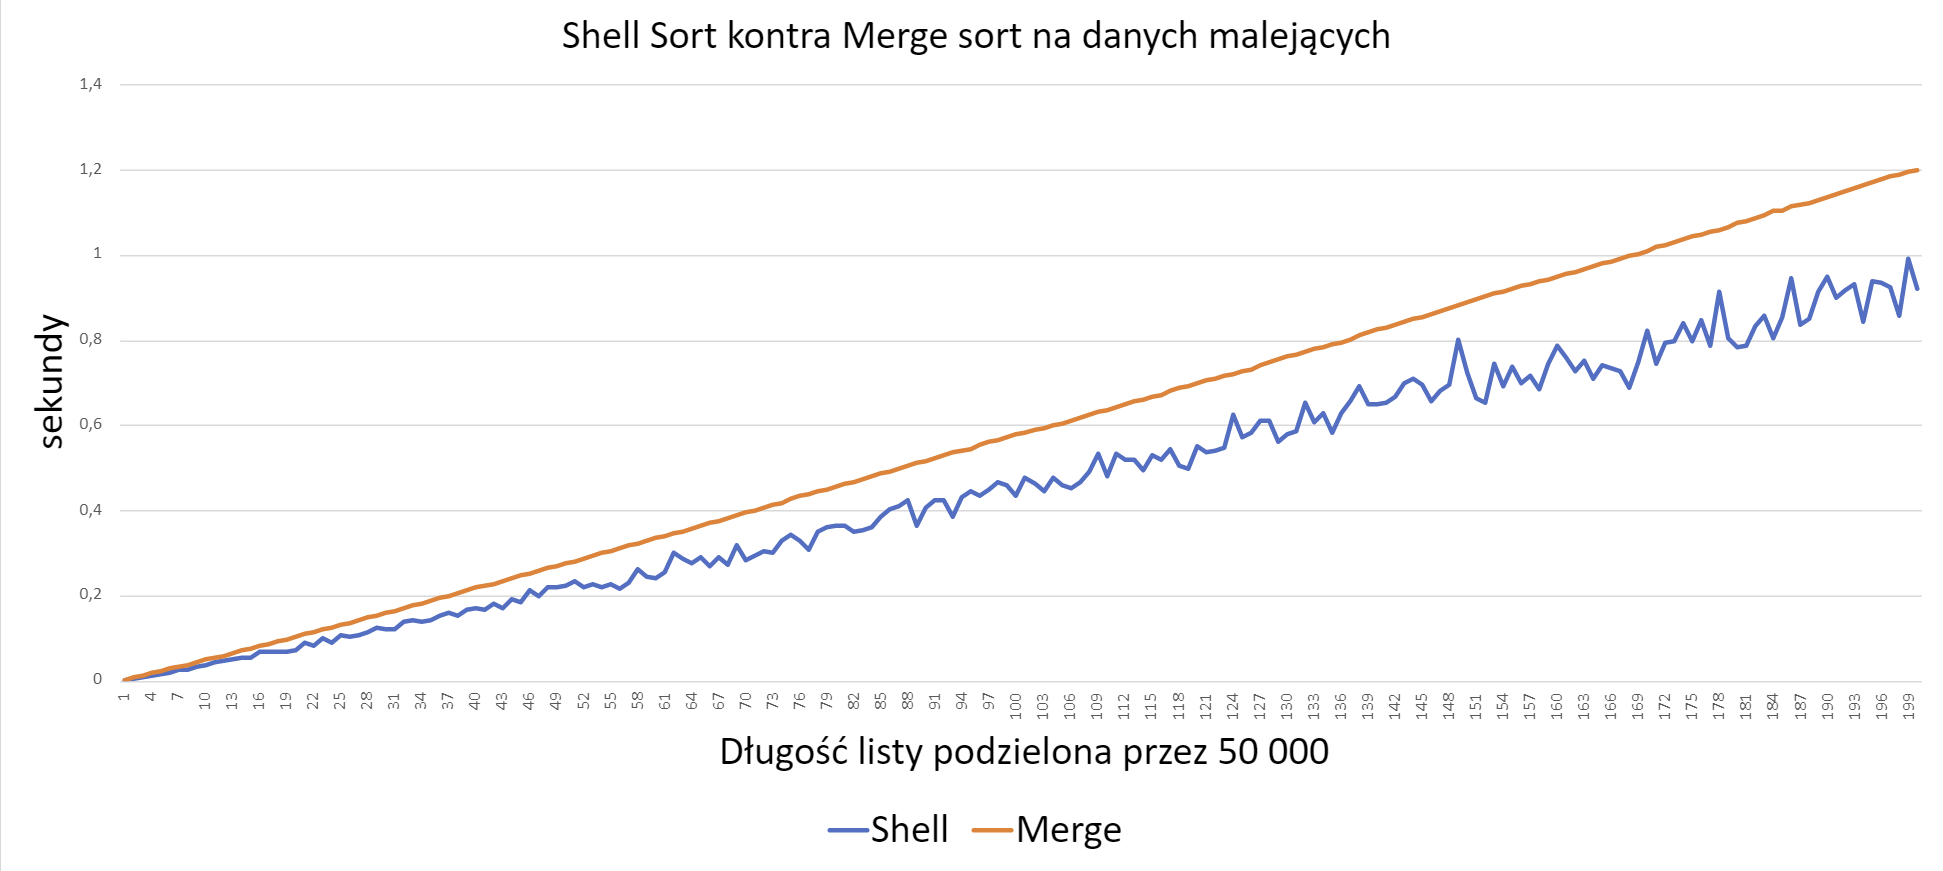
\includegraphics[scale = 0.23]{descend_f.png}\\
\caption{}
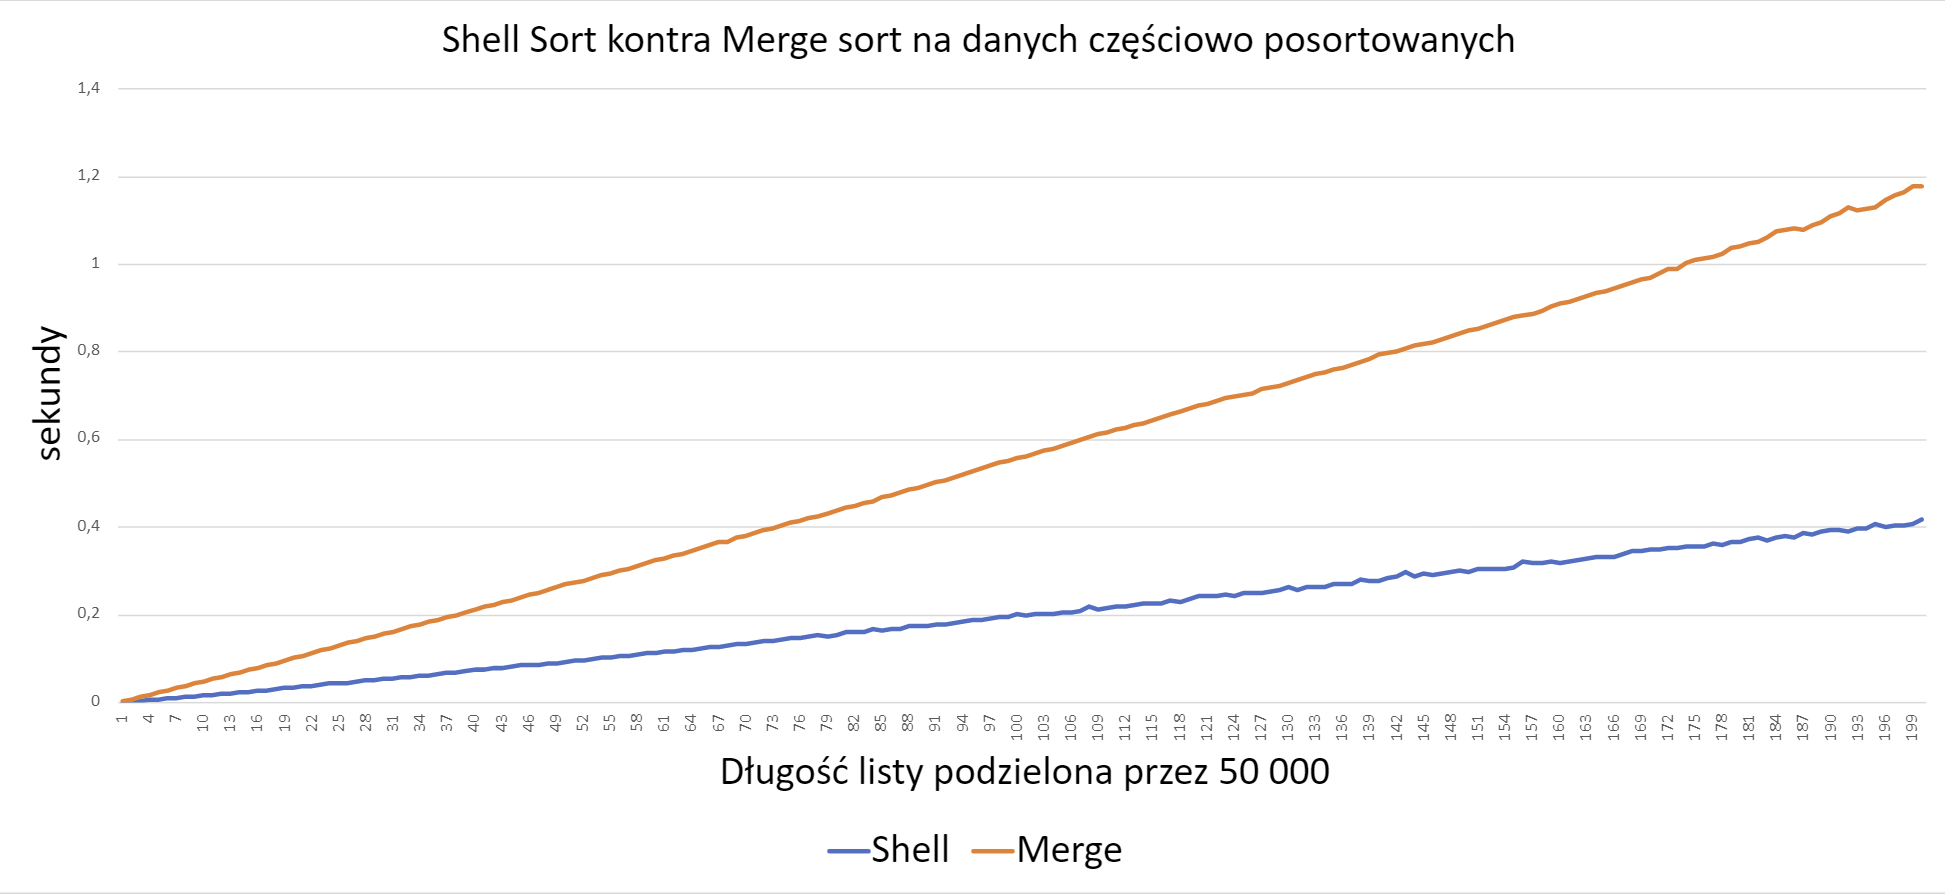
\includegraphics[scale = 0.23]{part-sort_f.png}\\
\end{figure}


\paragraph{}Jak możemy zauważyć z wykresów algorytm sortowania Shella, (w większości testowanych przypadków) działa w krótszym czasie od sortowania przez scalanie. Zasada ta jest prawdziwa dla zbiorów danych posortowanych rosnąco, zbiorów danych częściowo posortowanych oraz zbiorów danych posortowanych malejąco (gdzie różnica czasu wykonania jest stosunkowo niewielka). Wśród przeprowadzonych testów można zauważyć, że dla zbiorów danych losowych sortowanie przez scalanie wykonuje się w złożoności czasowej ${Nlog(N)}$ podczas, gdy sortowanie Shella zbliża się do swojej złożoności pesymistycznej - ${mN^k}$.

\break
\subsection{Dla jakich wielkości tablicy sortowanie Shella działa z porównywalną prędkością?}
Sortowanie Shella działa porównywalnie szybko do sortowania przez scalanie jedynie w przypadku sortowania zbiorów danych posortowanych malejąco (jak na wykresie 3). Przy takich zbiorach sortowanie przez scalanie, mimo że wolniejsze, jest wciąż stosunkowo bliskie sortowaniu Shella. Różnice te wynoszą co najwyżej 0,3 sekundy nawet dla największych z testowanych zbiorów.

\subsection{W jakich warunkach lepiej jest wykorzystać sortowanie Shell-a? Oraz do jakich zastosowań?}
\paragraph{} Sortowanie Shella sprawdzi się lepiej od sortowania przez scalanie kiedy:\\
• nasze dane są już częściowo posortowane,\\
• nie mamy do dyspozycji dodatkowej pamięci,\\
• zależy nam na prostocie działania algorytmu.
\paragraph{} 

Z uwagi na te różnice sortowanie Shella bywa stosowane zamiast sortowania szybkiego w implementacjach funkcji qsort z biblioteki standardowej języka C przeznaczonych dla systemów wbudowanych. Ponadto algorytm ten był również wykorzystywany w jądrze systemu operacyjnego Linux do 2017 oraz w programie bzip2, służącym do bezstratnej kompresji danych.


\end{document}
